\section{Aufbau}
\label{sec:Aufbau}
Allen Messungen liegt ein einfacher Aufbau zu Grunde. An einer Beamline des Elektronenspeicherrings DELTA
wird die im davorliegenden elektromagnetischen Undulator entstehende, Strahlung über einen Spiegel 
ausgekoppelt. Diese wird über zwei weitere Spiegel in eine dunkle Box geleitet. Dort durchquert der 
Lichtstrahl zuerst eine Blende dann eine Reihe von neutrale Dichte Filtern und eine weitere Blende bevor 
er auf eien Photomultiplier trifft. Dort werden einzelne Phottonen in elektrische Pulse umgewandelt.
Diese Pulse werden im weiteren mit unterschiedlichen Messinstrumenten aufgezeichnet und später ausgewertet.

\subsection{Der Undulator}
\label{sec:Undulator}
Zur Strahlungserzeugung wird der Undulator U255 auf der Nordostseite des Speicherrings genutzt.
Er besitztz $N_p= 17$ Perioden mit einer Periodenlänge von $\lambda_U=\SI{250}{\milli\meter}$.
Die Lücke zwischen den einzelnen Magneten beträgt $\SI{50}{\milli\meter}$.

\subsection{Optischer Aufbau}
\label{sec:Optik}
Die vom Undulator erzeugte Strahlung wird über drei Spiegel in eine dunkle Kiste geleitet. Der erste Spiegel
befindet sich in der verlängerten Undulatorachse und spiegelt den Strahl in horizontal-transversaler Richtung 
zu dieser in einen zweiten Spiegel, dieser dann wieder in einem $\SI{90}{\degree}$ Winkel auf Spiegel 3 in der
Blackbox. Nach dem dritten Spiegel passiert die Strahlung zunächst eine Blende, dann einen Bandpass welcher die 
Wellenlängen von $\SI{10000}{\nano\meter}$ bis $\SI{10000}{\nano\meter}$ passieren lässt. Anschließend folgt
ein Neutrale-Dichte-Filter, kurz: ND-Filter, welcher die Strahlung unabhängig von ihrer Wellenlänge um eine
bestimmte Zehnerpotzenz abschwächt. Hier wurden Filter mit einer Abschwächung von $10^7$ genutzt. Danach 
wird eine weitere Blende passiert, welche allerdings nur zum Schutz des empfindlichen Photomultipliers dient 
und wärend der Experimente stets vollständig geöffnet war. Wärend dem Betrieb des Aufbaus wurde die Kiste noch 
mit einem schwarzen Deckel verschlossen und das Licht im Labor ausgeschaltet um möglichst wenig Untergrundstrahlung
zu messsen. Siehe \autoref{fig:blackbox}.

\begin{figure}
  \centering
  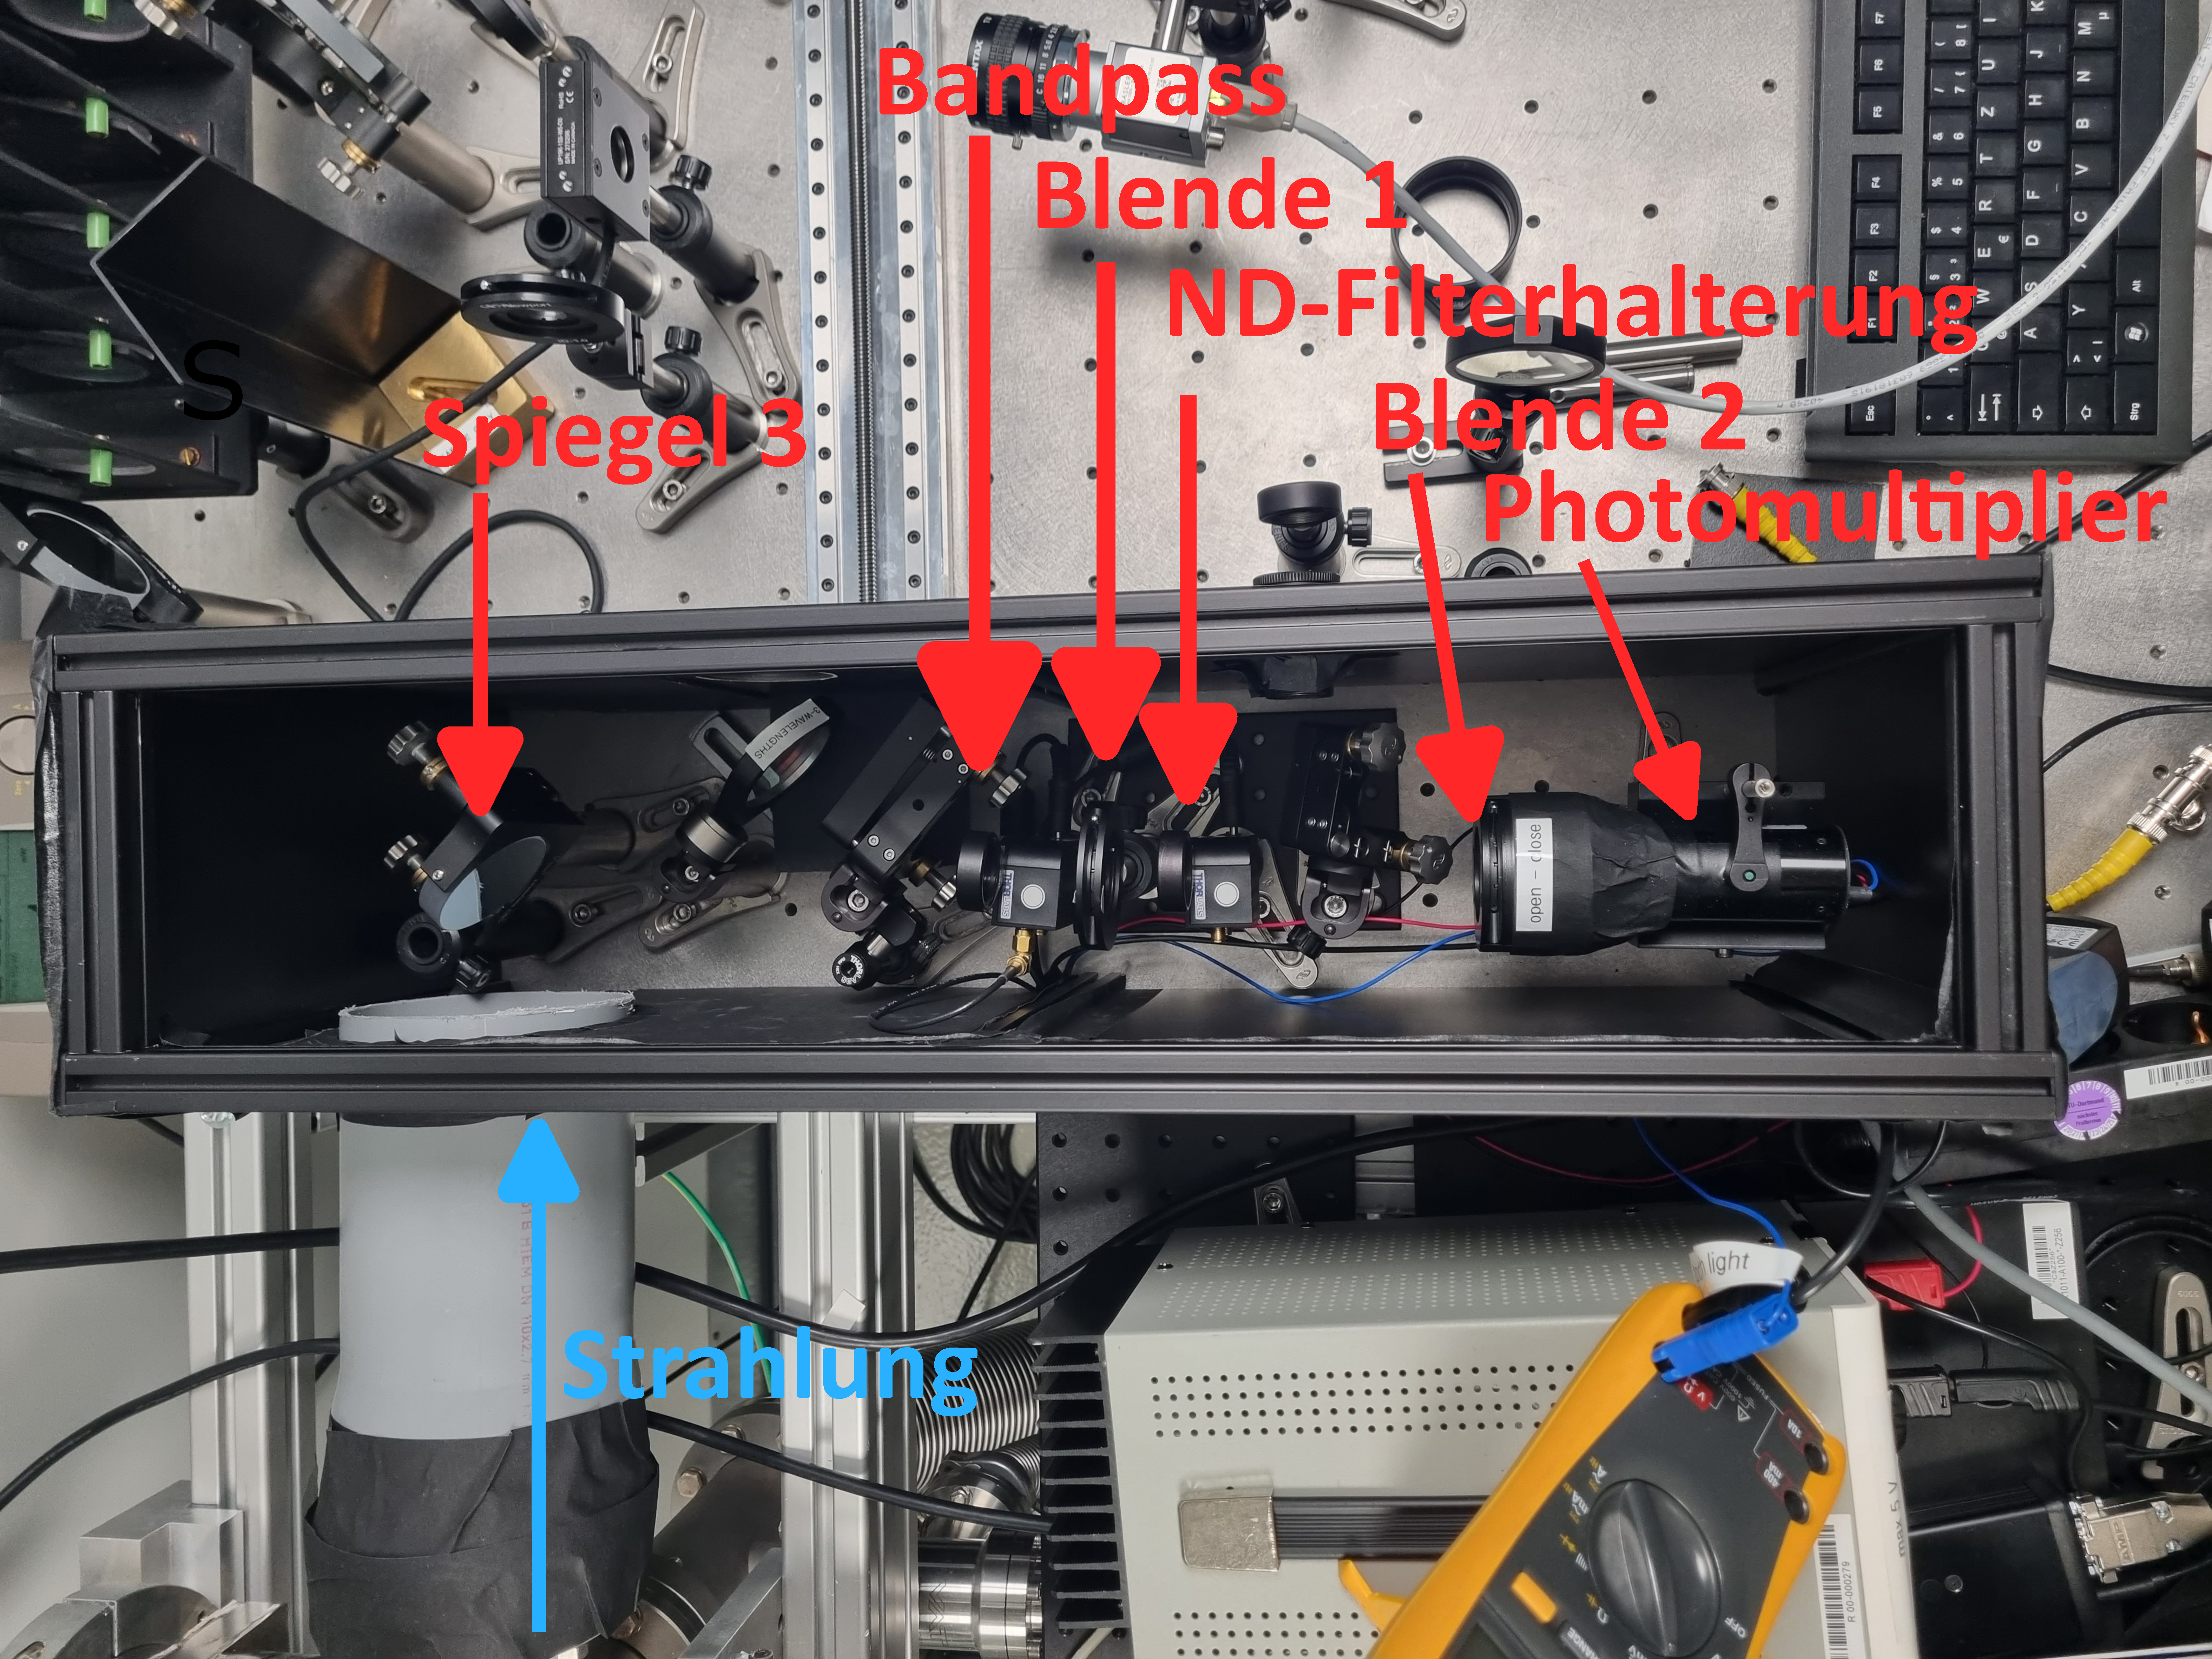
\includegraphics[width=16cm, height=12cm]{content/bilder/blackbox.pdf}
  \caption{Zu sehen ist der optische Aufbau. Nachdem die Strahlung in das Labor gespiegelt wurde wird sie durch
    eine Blende, einen Bandpass und einem ND-Filter abgeschwächt bevor sie auf den Photomultiplier trifft. }
  \label{fig:blackbox}
\end{figure}


\subsection{Der Photomultiplier}
\label{sec:Photomultiplier}
Für alle Experimente wurde der selbe Photomultiplier verwendet. Es handelt sich um einen Hamamatsu
H11870. Er arbeitet mit einer Spannung von lediglich fünf Volt und ist daher leicht zu handhaben.
Für jedes detektirte Photon gibt er einen Puls von etwa $\SI{9}{\nano\second}$ länge bei circa 
$\SI{2,2}{\volt}$ aus.



\subsection{Oszilloskop}
\label{sec:Oszilloskop}
Für die mit dem Oszilloskop durcheführten Messungen wurde ein Lecroy verwendet.

\subsection{TDC7201}
\label{sec:TDC}
Beim TDC7201 handelt es sich um einen Time to Digital Converter. Dieser besitzt einen Eingang für ein 
Start Signal und einen Eingang für ein Stop Signal. Der Chip misst die Zeit zwischen den steigenden oder 
fallenden Flanken der Signale. Die gemessenen Zeiten können dann über einen SPI Bus ausgelesen werden.
Das geschieht in diesem Aufbau durch einen Raspberry Pi. Dieses Verfahren funktioniert in nahezu Echtzeit. 
Daher kann mit diesem Aufbauleicht eine Füllstruktur errechnet und über das EPICS Protokoll im Netzwerk 
zur verfügung gestellt werden. Als Startsignal wird der DELTA Umlauftrigger genutzt. Als Stopsignal wird 
das Signal des Photomultipliers genutzt. Da es bei diesem Aufbau wahrscheinlicher ist Photonen von Bunches 
zu messen die als erstes nach dem Umlauftrigger Signal kommen, sollte das Umlauftriggersignal nach jeder 
Messung um zwei Nannosekunden verzögert werden um so alle Bunches über die Zeit gleich gut vermessen zu können.
Dazu wurde der Delaygenerator über das VXII Protokoll vom Raspberry Pi angesteuert.
Dieses Vorhaben scheiterte jedoch daran das der Delaygenerator nicht schnell genug umschalten konnte.
Daher müssen die gemessenen Signale später rechnerisch korrigiert werden. Dazu wurde ein Histogramm über 
meherere Umläufe erstellt und anhand dessen der Abfall der Messwahrscheinlichkeit bestimmt.

\begin{figure}
  \centering
  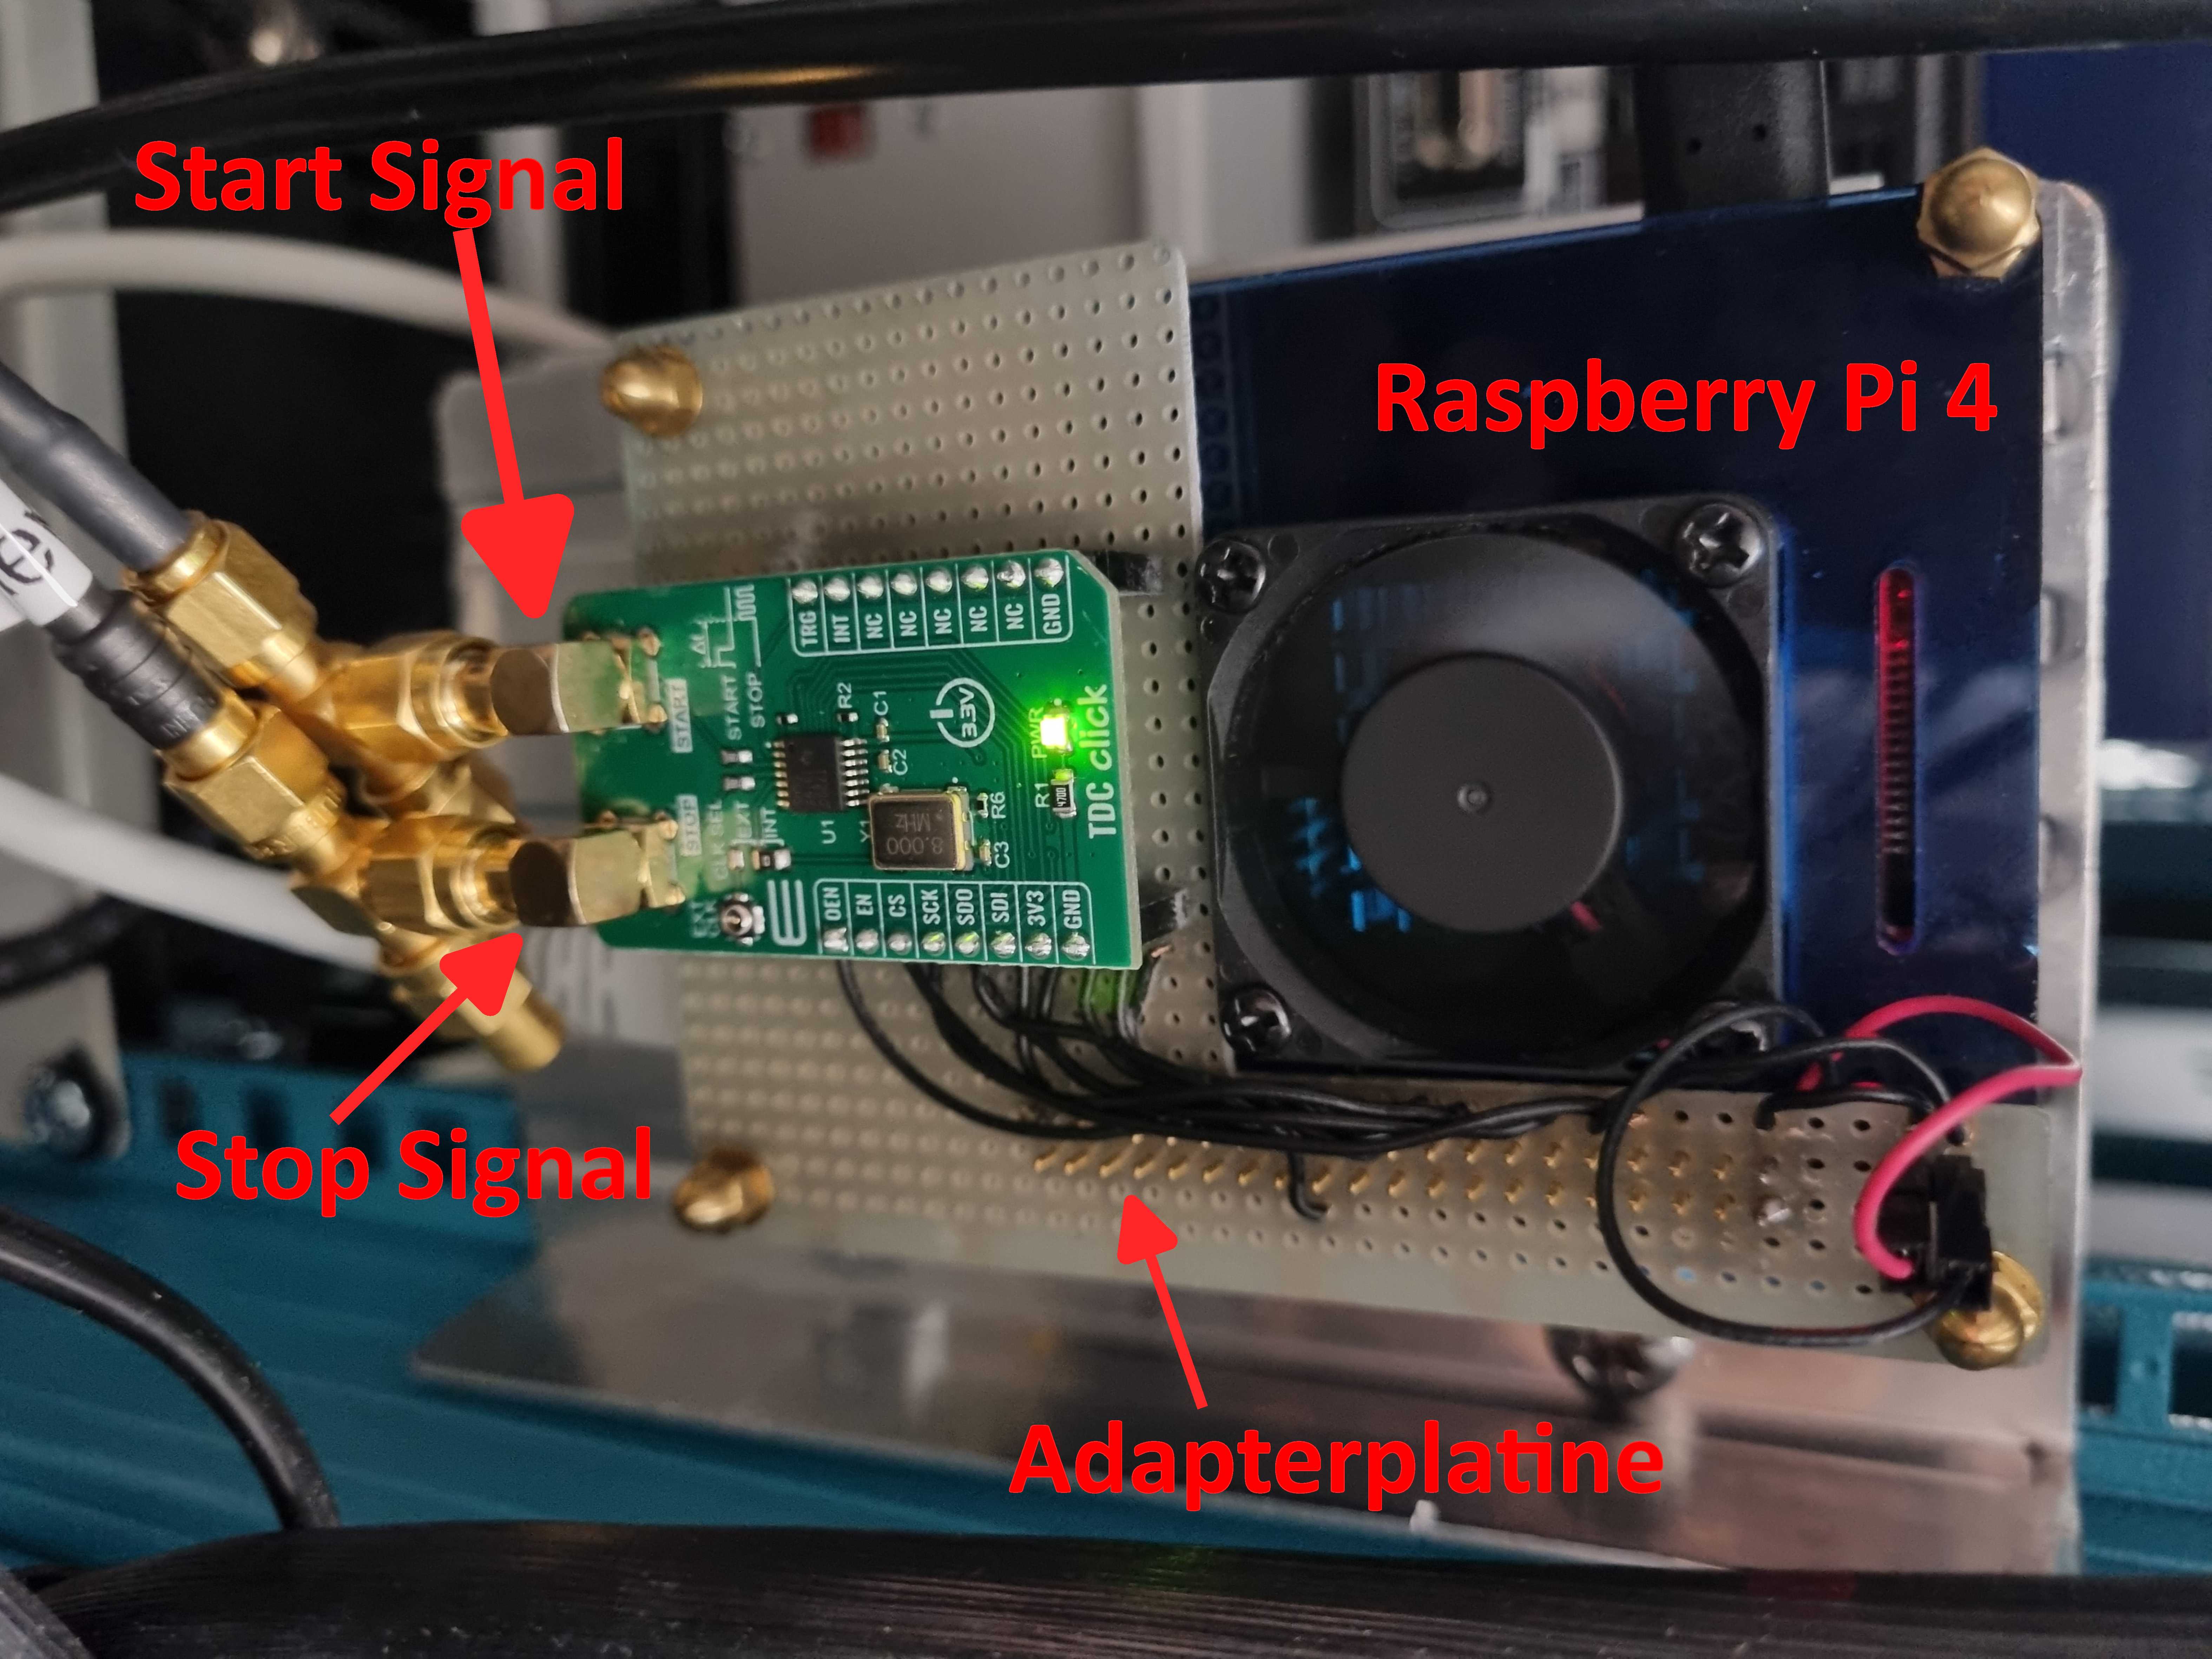
\includegraphics[width=16cm, height=12cm]{content/bilder/raspi.pdf}
  \caption{Auf dem Raspberry Pi befindset sich eine handgelöttete Adapterplatine welche fest mit dem Gehäuse
    des Raspberry Pis verschraupt ist und dessen GPIOs mit den Pins der Platine verbindet auf welcher der TDC7201
    aufgelötet ist. Start- und Stopsignal werden über koaxialkabel mit SMA Verbindern geliefert. Diese werden noch
    kurz vor dem Bord über ein T-Stück auf $\SI{50}{\ohm}$ abgeschlossen, da das TDC Board an sich eher einen offenen
    Abschluss darstellt.}
  \label{fig:raspi}
\end{figure}

\begin{figure}
  \centering
  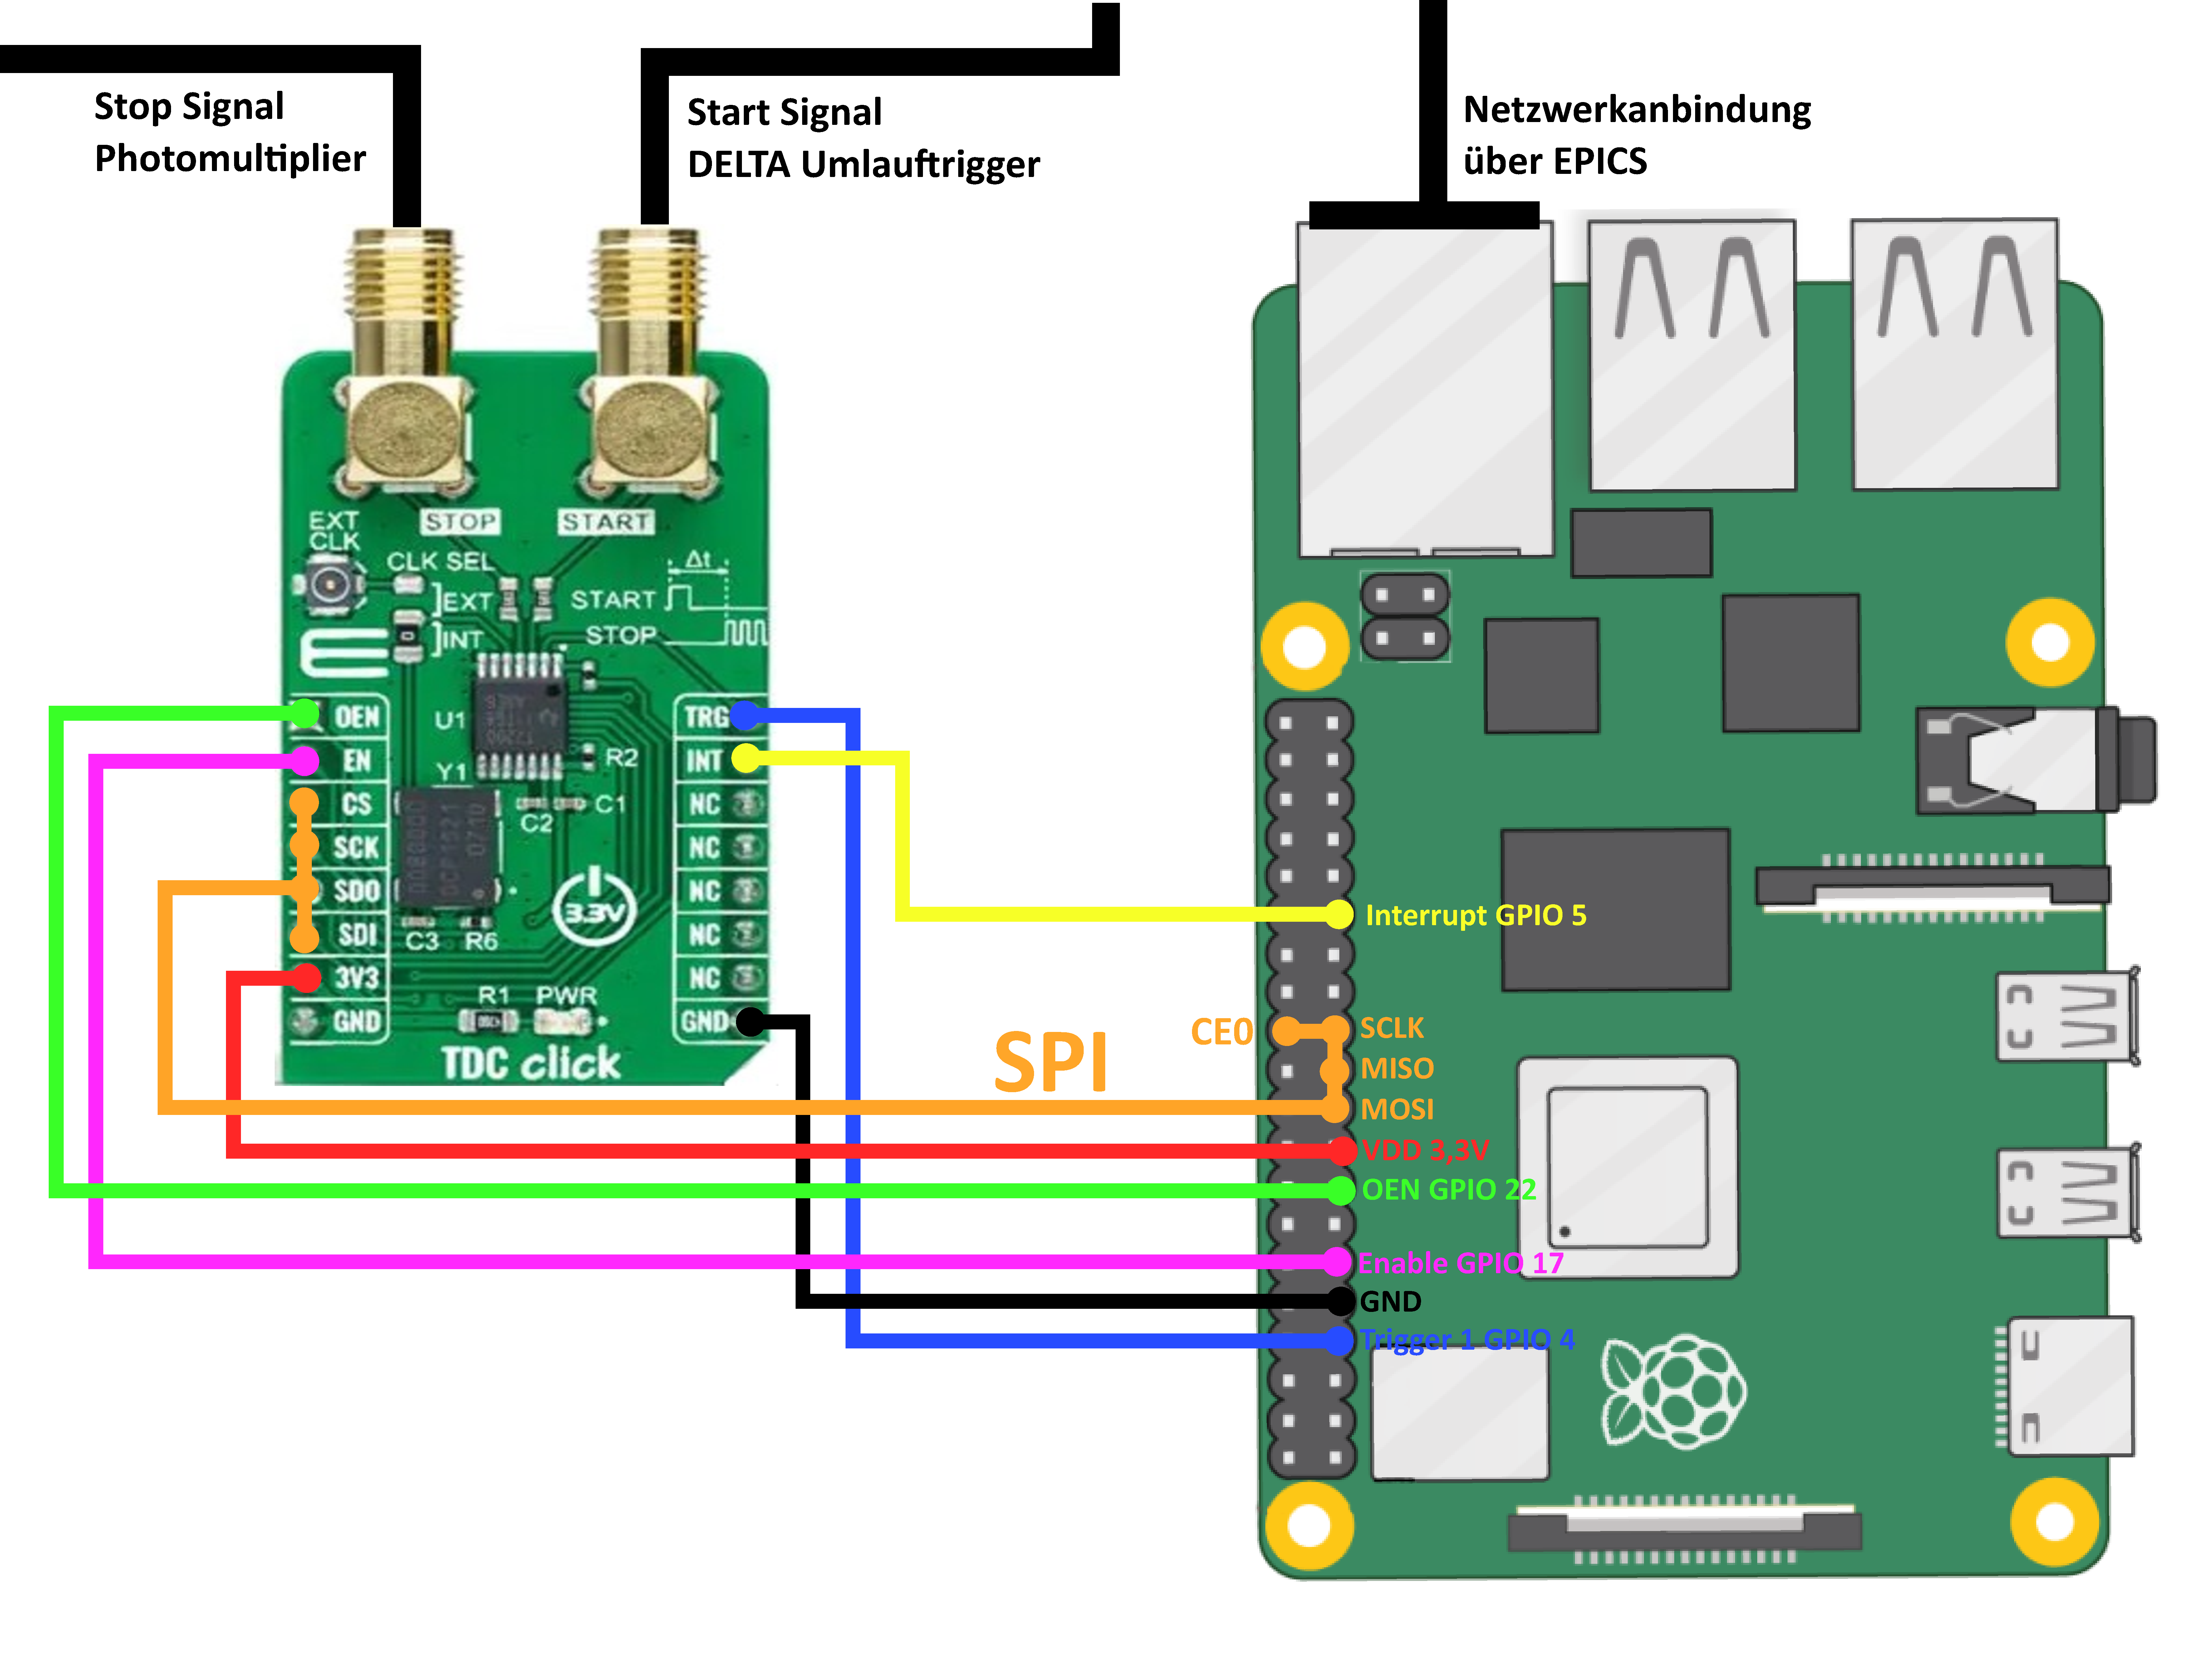
\includegraphics[width=16cm, height=12cm]{content/bilder/RaspiTdcSchaltung.pdf}
  \caption{Der Rspberry Pi ist über den SPI Bus (GPIO 10 MOSI, GPIO 9 MISO, GPIO 8 CE0 und GPIO 11 SCLK) mit dem TDC Board verbunden. 
    Zudem liefert der Raspberry Pi die benötigte Betriebsspannung von $V_{DD}=\SI{3,3}{\volt}$. Außerdem ist an GPIO 4 der
    Trigger-, an GPIO 17 der Enable-, an GPIO 22 der OEN und an GPIO 5 der Interrupteingang des TDC Boards angeschlossen. } 
  \label{fig:raspitdcschaltung}
\end{figure}

\subsection{Time Tagger}
\label{sec:TimeTagger}
Der Time Tagger ist ein dem in \autoref{sec:TDC} beschriebenen Aufbau ähnliches kommerzielles Produkt
der Firma Swabian Instruments.